\documentclass{article}

\usepackage{graphicx}
\usepackage{tikz}
\usepackage{tikzsymbols}
\usetikzlibrary{calc,patterns,shapes.geometric}
\pagestyle{empty}
\usepackage[margin=0pt]{geometry}
\geometry{papersize={14in,12in}}

\def\centerarc[#1](#2)(#3:#4:#5){\draw[#1] ($(#2)+({#5*cos(#3)},{#5*sin(#3)})$) arc (#3:#4:#5);}

\begin{document}
	\begin{figure}
		\centering
		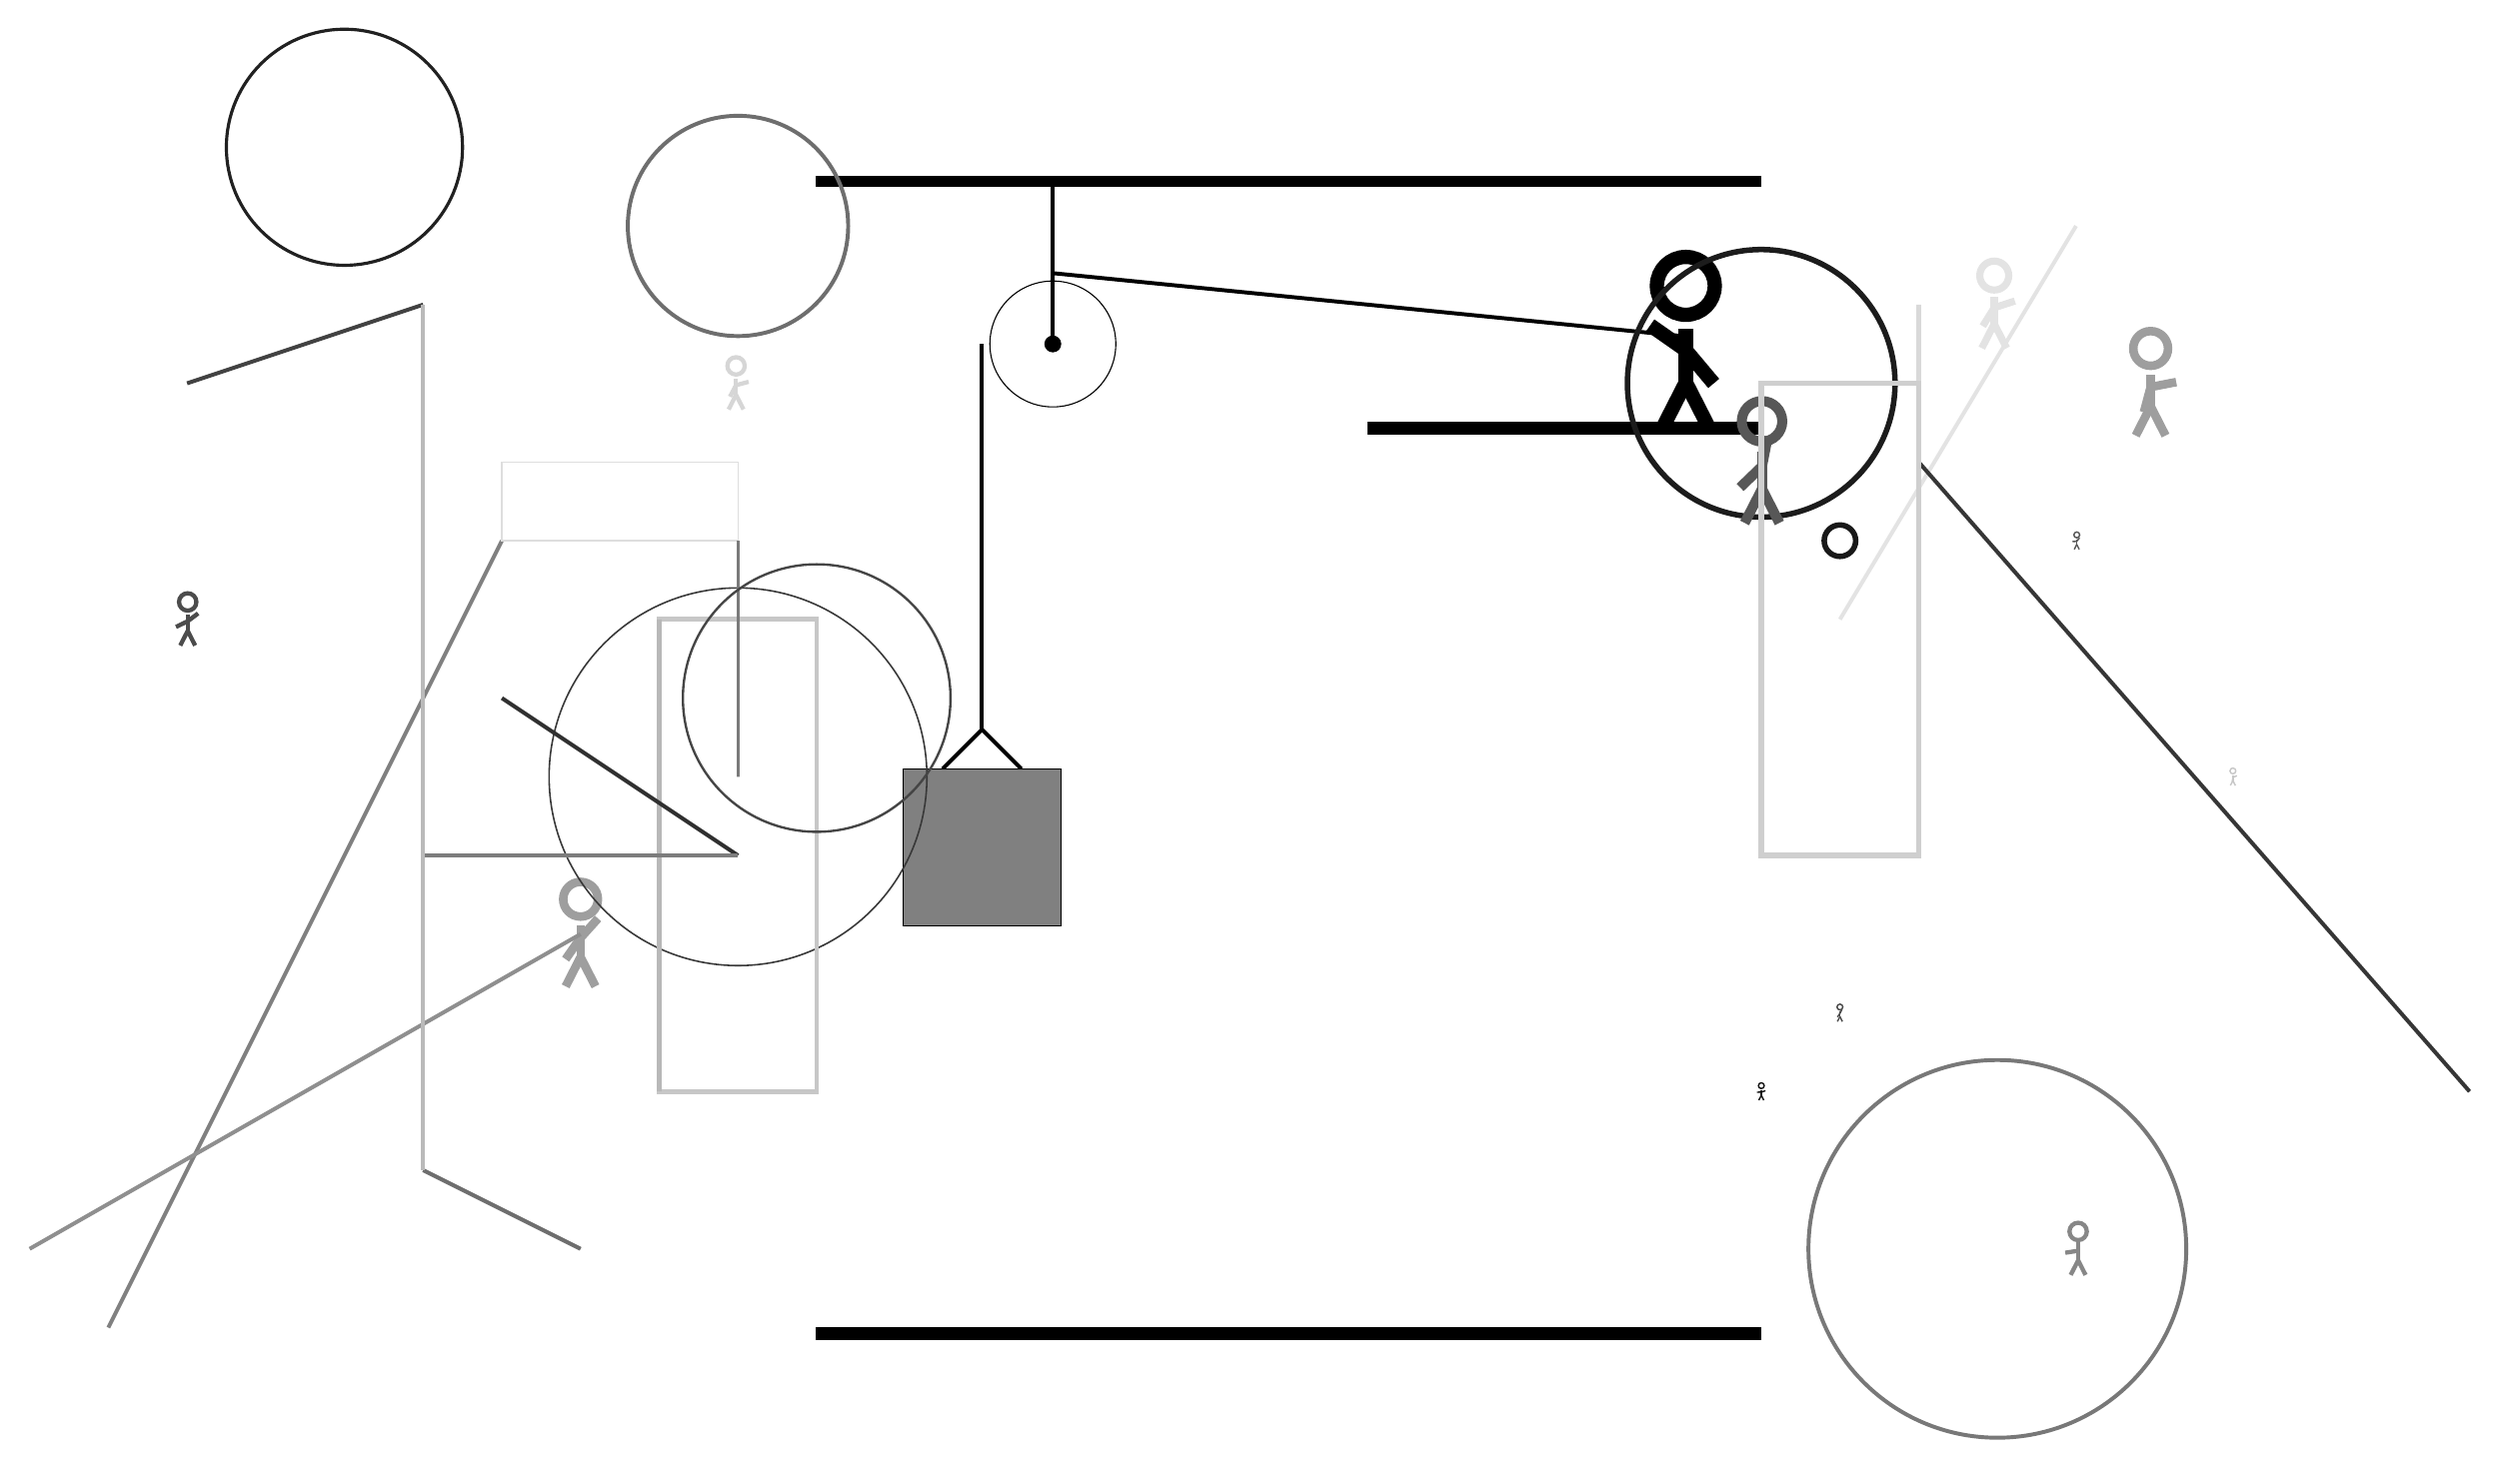
\begin{tikzpicture}
			%%%%% START %%%%%
			
			\draw[fill=black] (-2, 11.5) rectangle (10, 11.625);
			
			\draw (1, 9.5) circle (0.8);
			\draw[fill=black] (1, 9.5) circle (0.1);
			\draw[line width=0.5mm] (1, 11.5) -- (1, 9.5);
			
			\draw[line width=0.5mm](-0.4, 4.1) --  (0.1, 4.6) -- (0.6, 4.1);
			\draw[fill=black!50] (-0.9, 4.1) rectangle (1.1, 2.1);
			
			\draw[line width=0.5mm](0.1, 9.5) -- (0.1, 4.6);
			\centerarc[line width=0.5mm](1, 9.5)(90:180:0.9)
			\draw[line width=0.5mm](1, 10.4) -- (9, 9.6);
			
			\node at (9, 9.5) {\Strichmaxerl[10][-35][-50]};
			\draw[fill=black] (5, 8.5) rectangle (10, 8.35);
			
			\node[line width=0.2mm, color=black!38] at (-5, 2) {\Strichmaxerl[6][55][48]};
			
			\node[line width=0.3mm, color=black!11] at (13, 10) {\Strichmaxerl[5][58][18]};
			\draw [line width=0.7mm, color=black!89](10, 9) circle (1.7);
			\draw[line width=0.5mm, color=black!11](11, 6) -- (14, 11);
			
			\draw[line width=0.5mm, color=black!50](-6, 7) -- (-11, -3);
			\draw [line width=0.5mm, color=black!53](13, -2) circle (2.4);
			
			\draw[line width=0.5mm, color=black!57](-7, -1) -- (-5, -2);
			
			\node[line width=0.5mm, color=black!22] at (16, 4) {\Strichmaxerl[1][82][22]};
			\draw [line width=0.7mm, color=black!90](11, 7) circle (0.2);
			\draw[line width=0.5mm, color=black!16] (10, 5) rectangle (10, 3);
			\draw[line width=0.3mm, color=black!98] (-2, 0) rectangle (-2, 0);
			\draw [line width=0.5mm, color=black!57](-3, 11) circle (1.4);
			\draw [line width=0.4mm, color=black!63](-2, 0) circle (0.0);
			\node[line width=0.4mm, color=black!66] at (14, 7) {\Strichmaxerl[1][4][51]};
			\draw [line width=0.2mm, color=black!78](-3, 4) circle (2.4);
			\node[line width=0.4mm, color=black!92] at (10, 0) {\Strichmaxerl[1][2][19]};
			
			\draw[line width=0.6mm, color=black!15] (12, 10) rectangle (12, 6);
			\draw[line width=0.2mm, color=black!13] (-3, 8) rectangle (-6, 7);
			\draw [line width=0.4mm, color=black!87](-8, 12) circle (1.5);
			
			\node[line width=0.3mm, color=black!70] at (-10, 6) {\Strichmaxerl[3][26][37]};
			\draw[line width=0.6mm, color=black!22] (-2, 6) rectangle (-4, 0);
			
			\draw[line width=0.5mm, color=black!74](-7, 10) -- (-10, 9);
			
			\draw[line width=0.5mm, color=black!44](-5, 2) -- (-12, -2);
			\draw[line width=0.4mm, color=black!52] (-3, 4) rectangle (-3, 7);
			\draw[line width=0.6mm, color=black!28] (-4, 6) rectangle (-4, 0);
			\node[line width=0.3mm, color=black!71] at (11, 1) {\Strichmaxerl[1][55][63]};
			\draw[line width=0.5mm, color=black!81](-3, 3) -- (-6, 5);
			\node[line width=0.7mm, color=black!38] at (15, 9) {\Strichmaxerl[6][75][11]};
			
			\node[line width=0.6mm, color=black!66] at (10, 8) {\Strichmaxerl[7][44][79]};
			\draw [line width=0.3mm, color=black!73](-2, 5) circle (1.7);
			\draw[line width=0.5mm, color=black!79](12, 8) -- (19, 0);
			
			\draw[line width=0.7mm, color=black!19] (10, 3) rectangle (12, 9);
			\node[line width=0.6mm, color=black!47] at (14, -2) {\Strichmaxerl[3][9][90]};
			
			\node[line width=0.3mm, color=black!16] at (-3, 9) {\Strichmaxerl[3][62][15]};
			\draw[line width=0.5mm, color=black!51](-3, 3) -- (-7, 3);
			\draw[line width=0.5mm, color=black!27](-7, 10) -- (-7, -1);
			
			\draw[fill=black] (-2, -3) rectangle (10, -3.15);
			
			%%%%% END %%%%%
		\end{tikzpicture}
	\end{figure}	
\end{document}